\documentclass[12pt]{article}

% Page format
\usepackage[margin=1in]{geometry}

% Math packages and custom commands 
\usepackage{framed, tikz}
\usepackage[utf8]{inputenc}
\usepackage{mathtools,amsthm}
\usepackage{enumitem,amssymb}
\usepackage{hyperref}

\newtheoremstyle{case}{}{}{}{}{}{:}{ }{}
\theoremstyle{case}
\newtheorem{case}{Case}
\DeclareMathOperator{\R}{\mathbb{R}}
\DeclareMathOperator{\E}{\mathbb{E}}
\DeclareMathOperator{\Var}{\text{Var}}
\DeclareMathOperator{\Cov}{\text{Cov}}
\newcommand{\bvec}[1]{\mathbf{#1}}
\renewcommand{\P}{\mathbb{P}}
\newcommand{\norm}[2][2]{\| #2\|_{#1}}
\newcommand{\maxnorm}[2][\infty]{\| #2\|_{#1}}
\newcommand{\note}[1]{\noindent{[\textbf{NOTE:} #1]}}
\newcommand{\hint}[1]{\noindent{[\textbf{HINT:} #1]}}
\newcommand{\recall}[1]{\noindent{[\textbf{RECALL:} #1]}}

\definecolor{shadecolor}{gray}{0.9}


\begin{document}

\begin{center}
{\Large CSCE 580, Fall 2020 \\ Assignment 3}

\begin{tabular}{rl}
Username: & primiani@email.sc.edu \\
Name: & Jack Primiani \\
\end{tabular}
\end{center}

By turning in this assignment, I agree by the honor code of USC Columbia.

\paragraph{Submission.}
You need to submit the following files to Blackboard:
\begin{itemize}
    \item A pdf file named as assignment3\_$\langle username \rangle$.pdf, where you replace $\langle username \rangle$ with your email username. This pdf file contains your anwsers to Problems 1 and 2: Edit the assignment3.tex file to fill in your answers for Problems 1 and 2, and submit the pdf file generated from the edited tex file. 
    \item A zip file named as assignment3\_$\langle username \rangle$.zip, where you replace $\langle username \rangle$ with your email username.
    This zip file contains the single file of multiAgents.py specified in Problem 3.
    \item A html file named as assignment3\_$\langle username \rangle$.html, where you replace $\langle username \rangle$ with your email username. The html file contains the autograder's results. Please see Problem 3 for details.
\end{itemize}

\section*{Problem 1 [10 pt]: Two-player zero-sum games}
Consider the zero-sum game tree shown below. Triangles that point up, such as at the top node (root), represent choices for the maximizing player; triangles that point down represent choices for the minimizing player.
\begin{figure}[h]
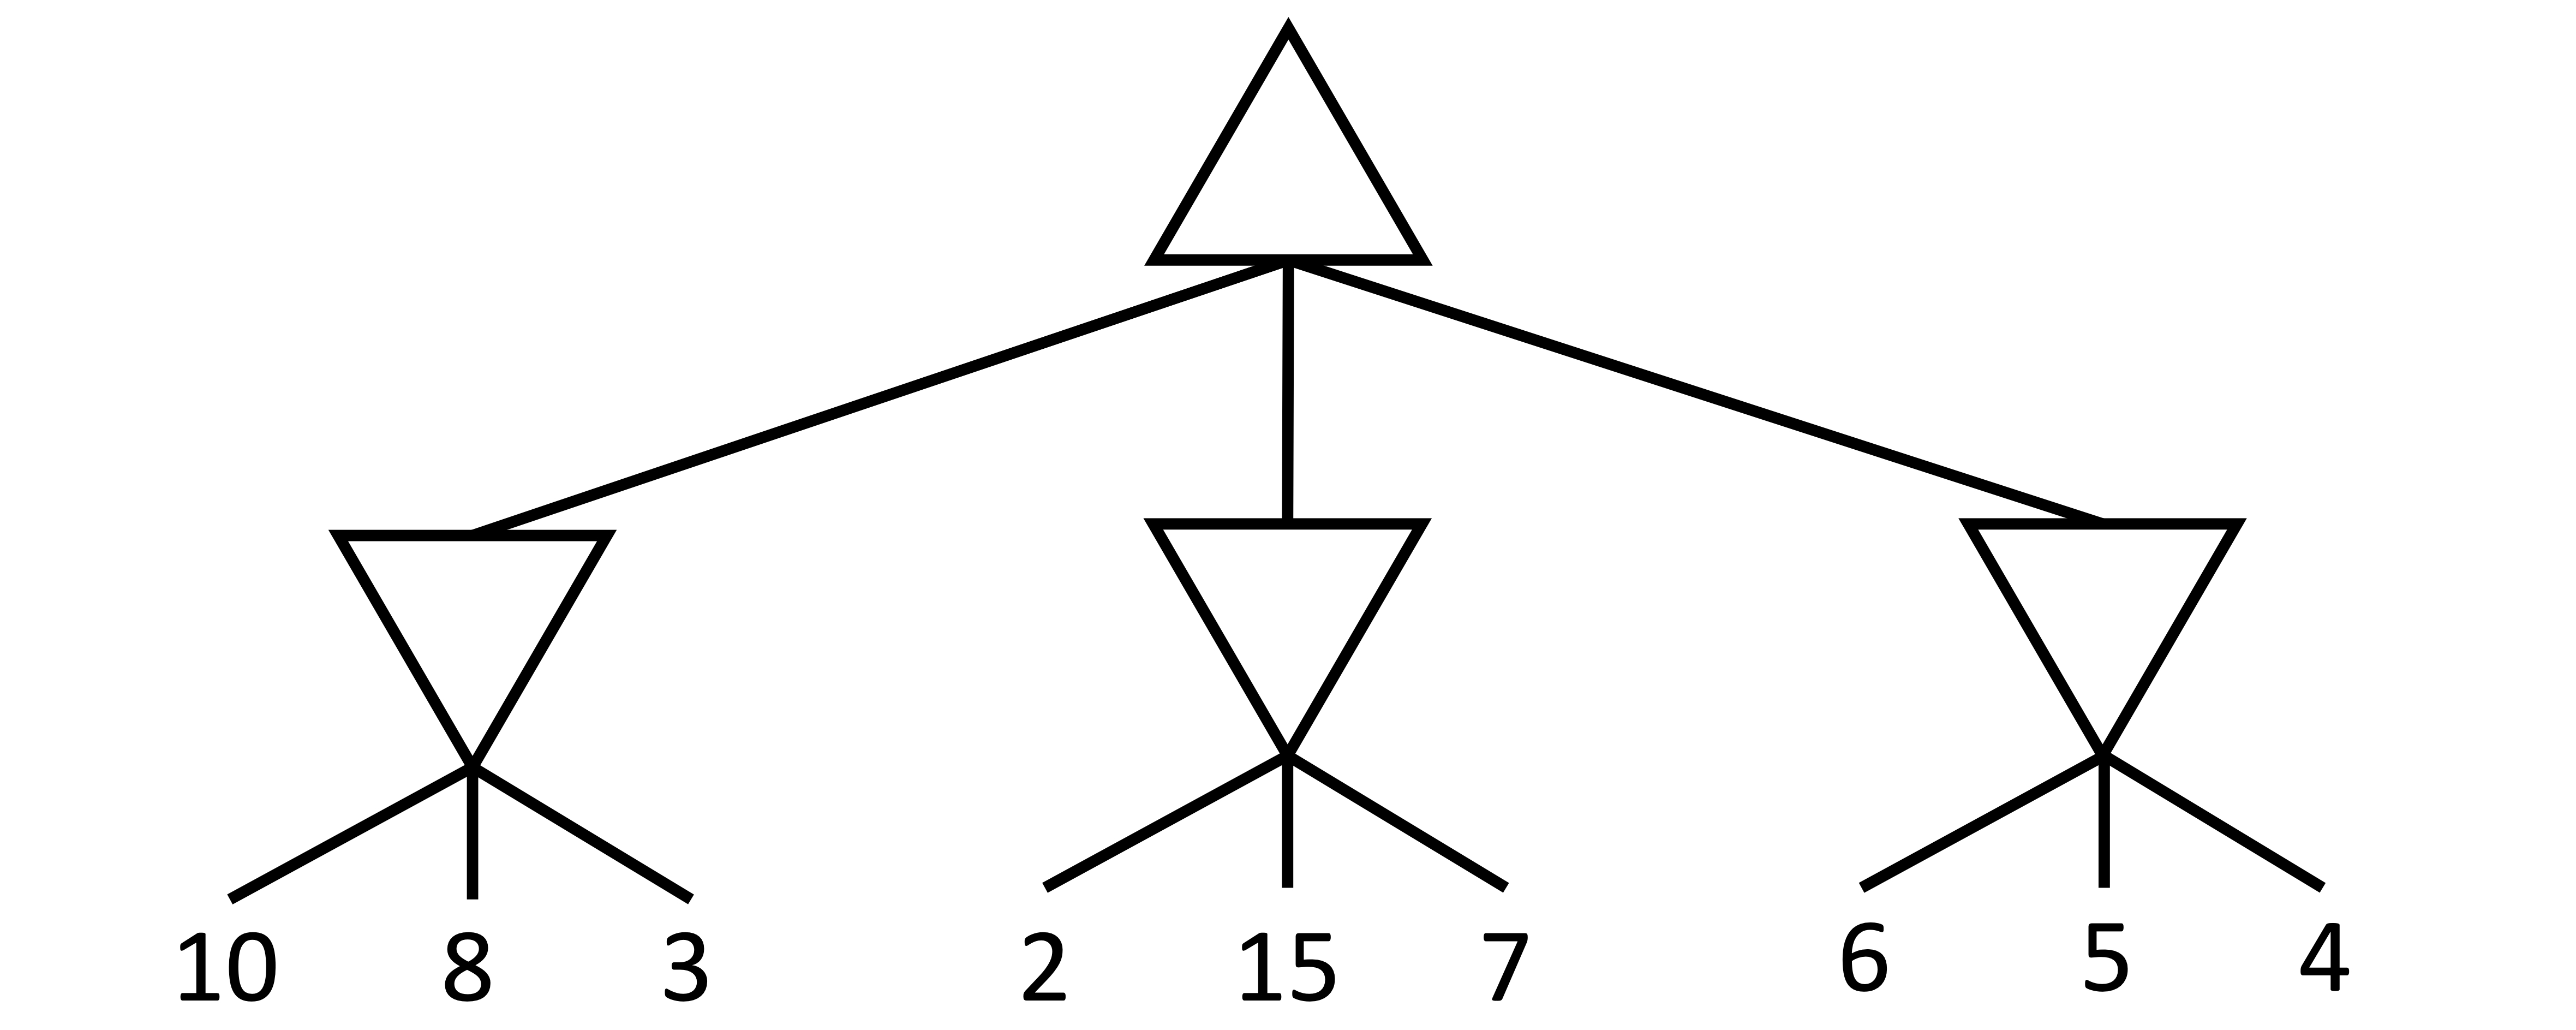
\includegraphics[width=.7\textwidth]{assignment3_1.jpg}
\centering
\end{figure}
 
    
\begin{enumerate} [label=(\alph*)]
    \item
    What are the minimax values of each of the four nodes?
    
P, Q, R are min-nodes:

        U(P)=min {10, 8, 3}

        U(Q)=min {2, 15, 7}

        U(R)=min {6, 5, 4}

S is a max-node:

  U(S)={3,2,4} = 4






    \item
    Which leaves can be pruned from the game tree above through alpha-beta pruning? If no nodes can be pruned, explain why not. Assume the search goes from left to right: when choosing which child to visit first, choose the left-most unvisited child.
   
No nodes can be pruned. There will always be the possibility that some leaf further down the branch will have a very high value, which increases the overall average value.
    
    \item 
    Again,consider the same game tree,except that now,instead of a minimizing player,we have a chance node that will select one of the three values uniformly at random. What are the expectimax value of each of the four nodes?
   
P, Q, R are children of S:

        Expectimax of P = 7

        Expectimax of Q = 8

        Expectimax of R = 5

        Expectimax of S = 8

\end{enumerate}

\newpage
\section*{Problem 2 [20 pt]: One Wish Pacman}
Pacman has a special power: {\em once} in the entire game when a ghost is selecting an action, Pacman can make the ghost choose any desired action instead of the min-action which the ghost would normally take. {\em The ghosts know about this special power and act accordingly.}

Similar to the minimax algorithm, where the value of each node is determined by the game subtree hanging from that node, we define a value pair $(u,v)$ for each node: $u$ is the value of the subtree if the power is not used in that subtree; $v$ is the value of the subtree if the power is used once in that subtree. For example, in the below subtree with values (-3, 5), if Pacman does not use the power, the ghost acting as a minimizer would choose -3; however, with the special power, Pacman can make the ghost choose the value more desirable to Pacman, in this case 5.

{\em Reminder:} Being allowed to use the power once during the game is different from being allowed to use the power in only one node in the game tree below. For example, if Pacman’s strategy was to always use the special power on the second ghost then that would only use the power once during execution of the game, but the power would be used in four possible different nodes in the game tree.

For the terminal states we set $u = v = $ Utility(state).

\begin{figure}[h]
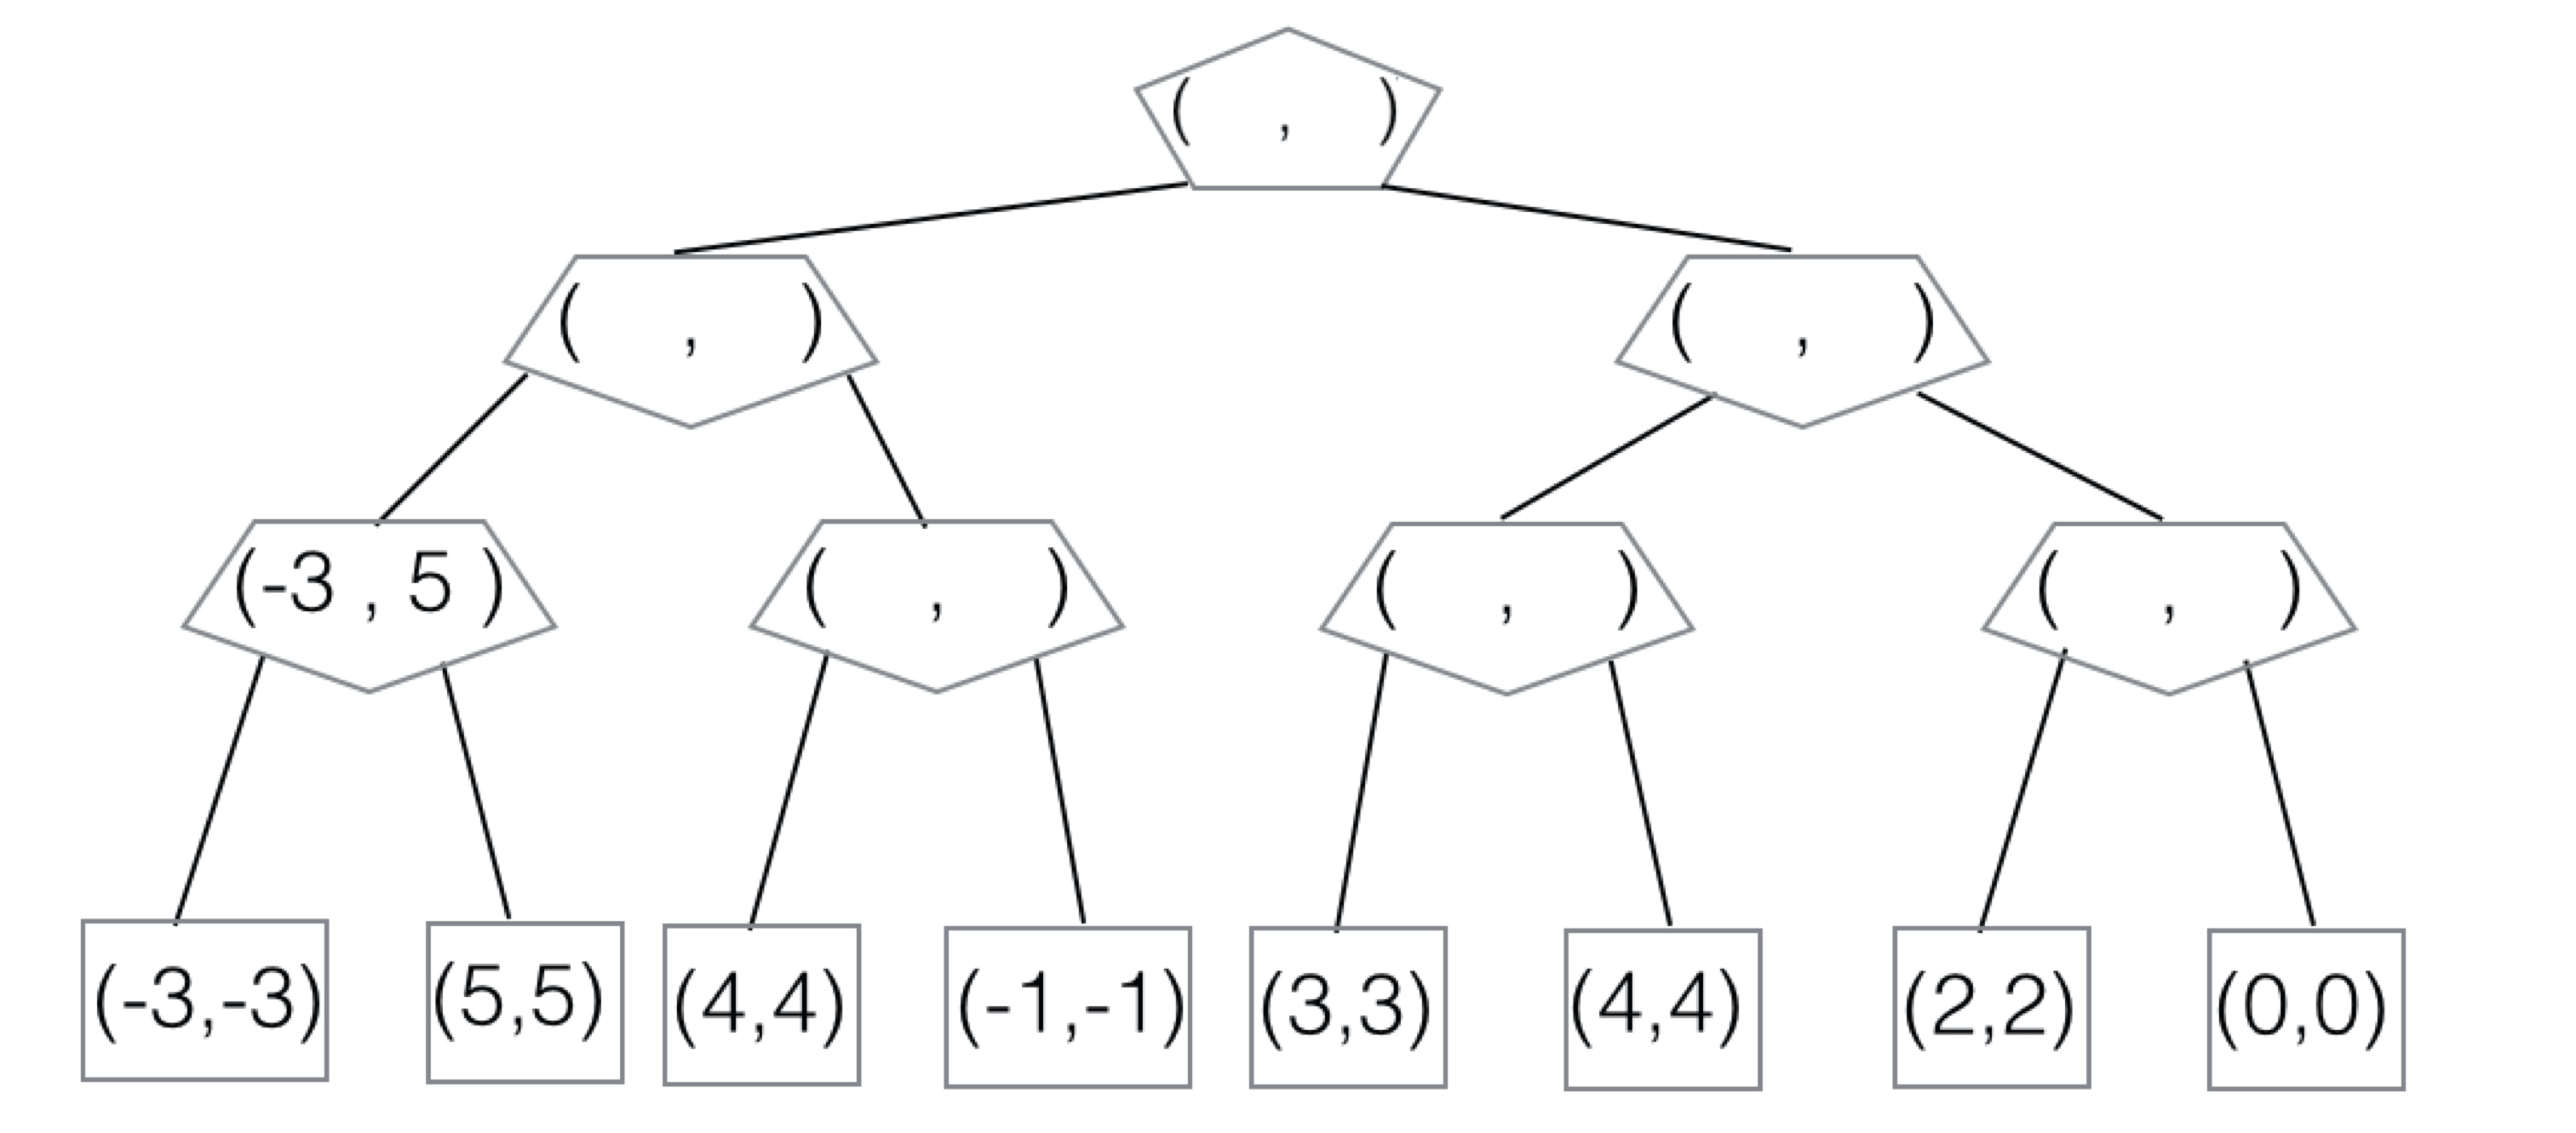
\includegraphics[width=1.\textwidth]{assignment3_2.jpg}
\centering
\end{figure}
 
    
\begin{enumerate} [label=(\alph*)]
    \item
    Find the $(u, v)$ values in the modified minimax tree above. Pacman is the root and there are two ghosts.
    
~~~~~~~~~~~~~(0,4)

~~~~~(-3,4)~~~~~~~~~~~~~(0,3)

(-3,5)~~~~~(-1,4)~~~(3,4)~~~~(0,2)

    
    \item Complete the algorithm below, which is a modification of the minimax algorithm, to work in the general case: Pacman can use the power at most once in the game but Pacman and ghosts can have multiple turns in the game. Briefly explain your completion of the two blanks.
    \begin{figure}[h]
    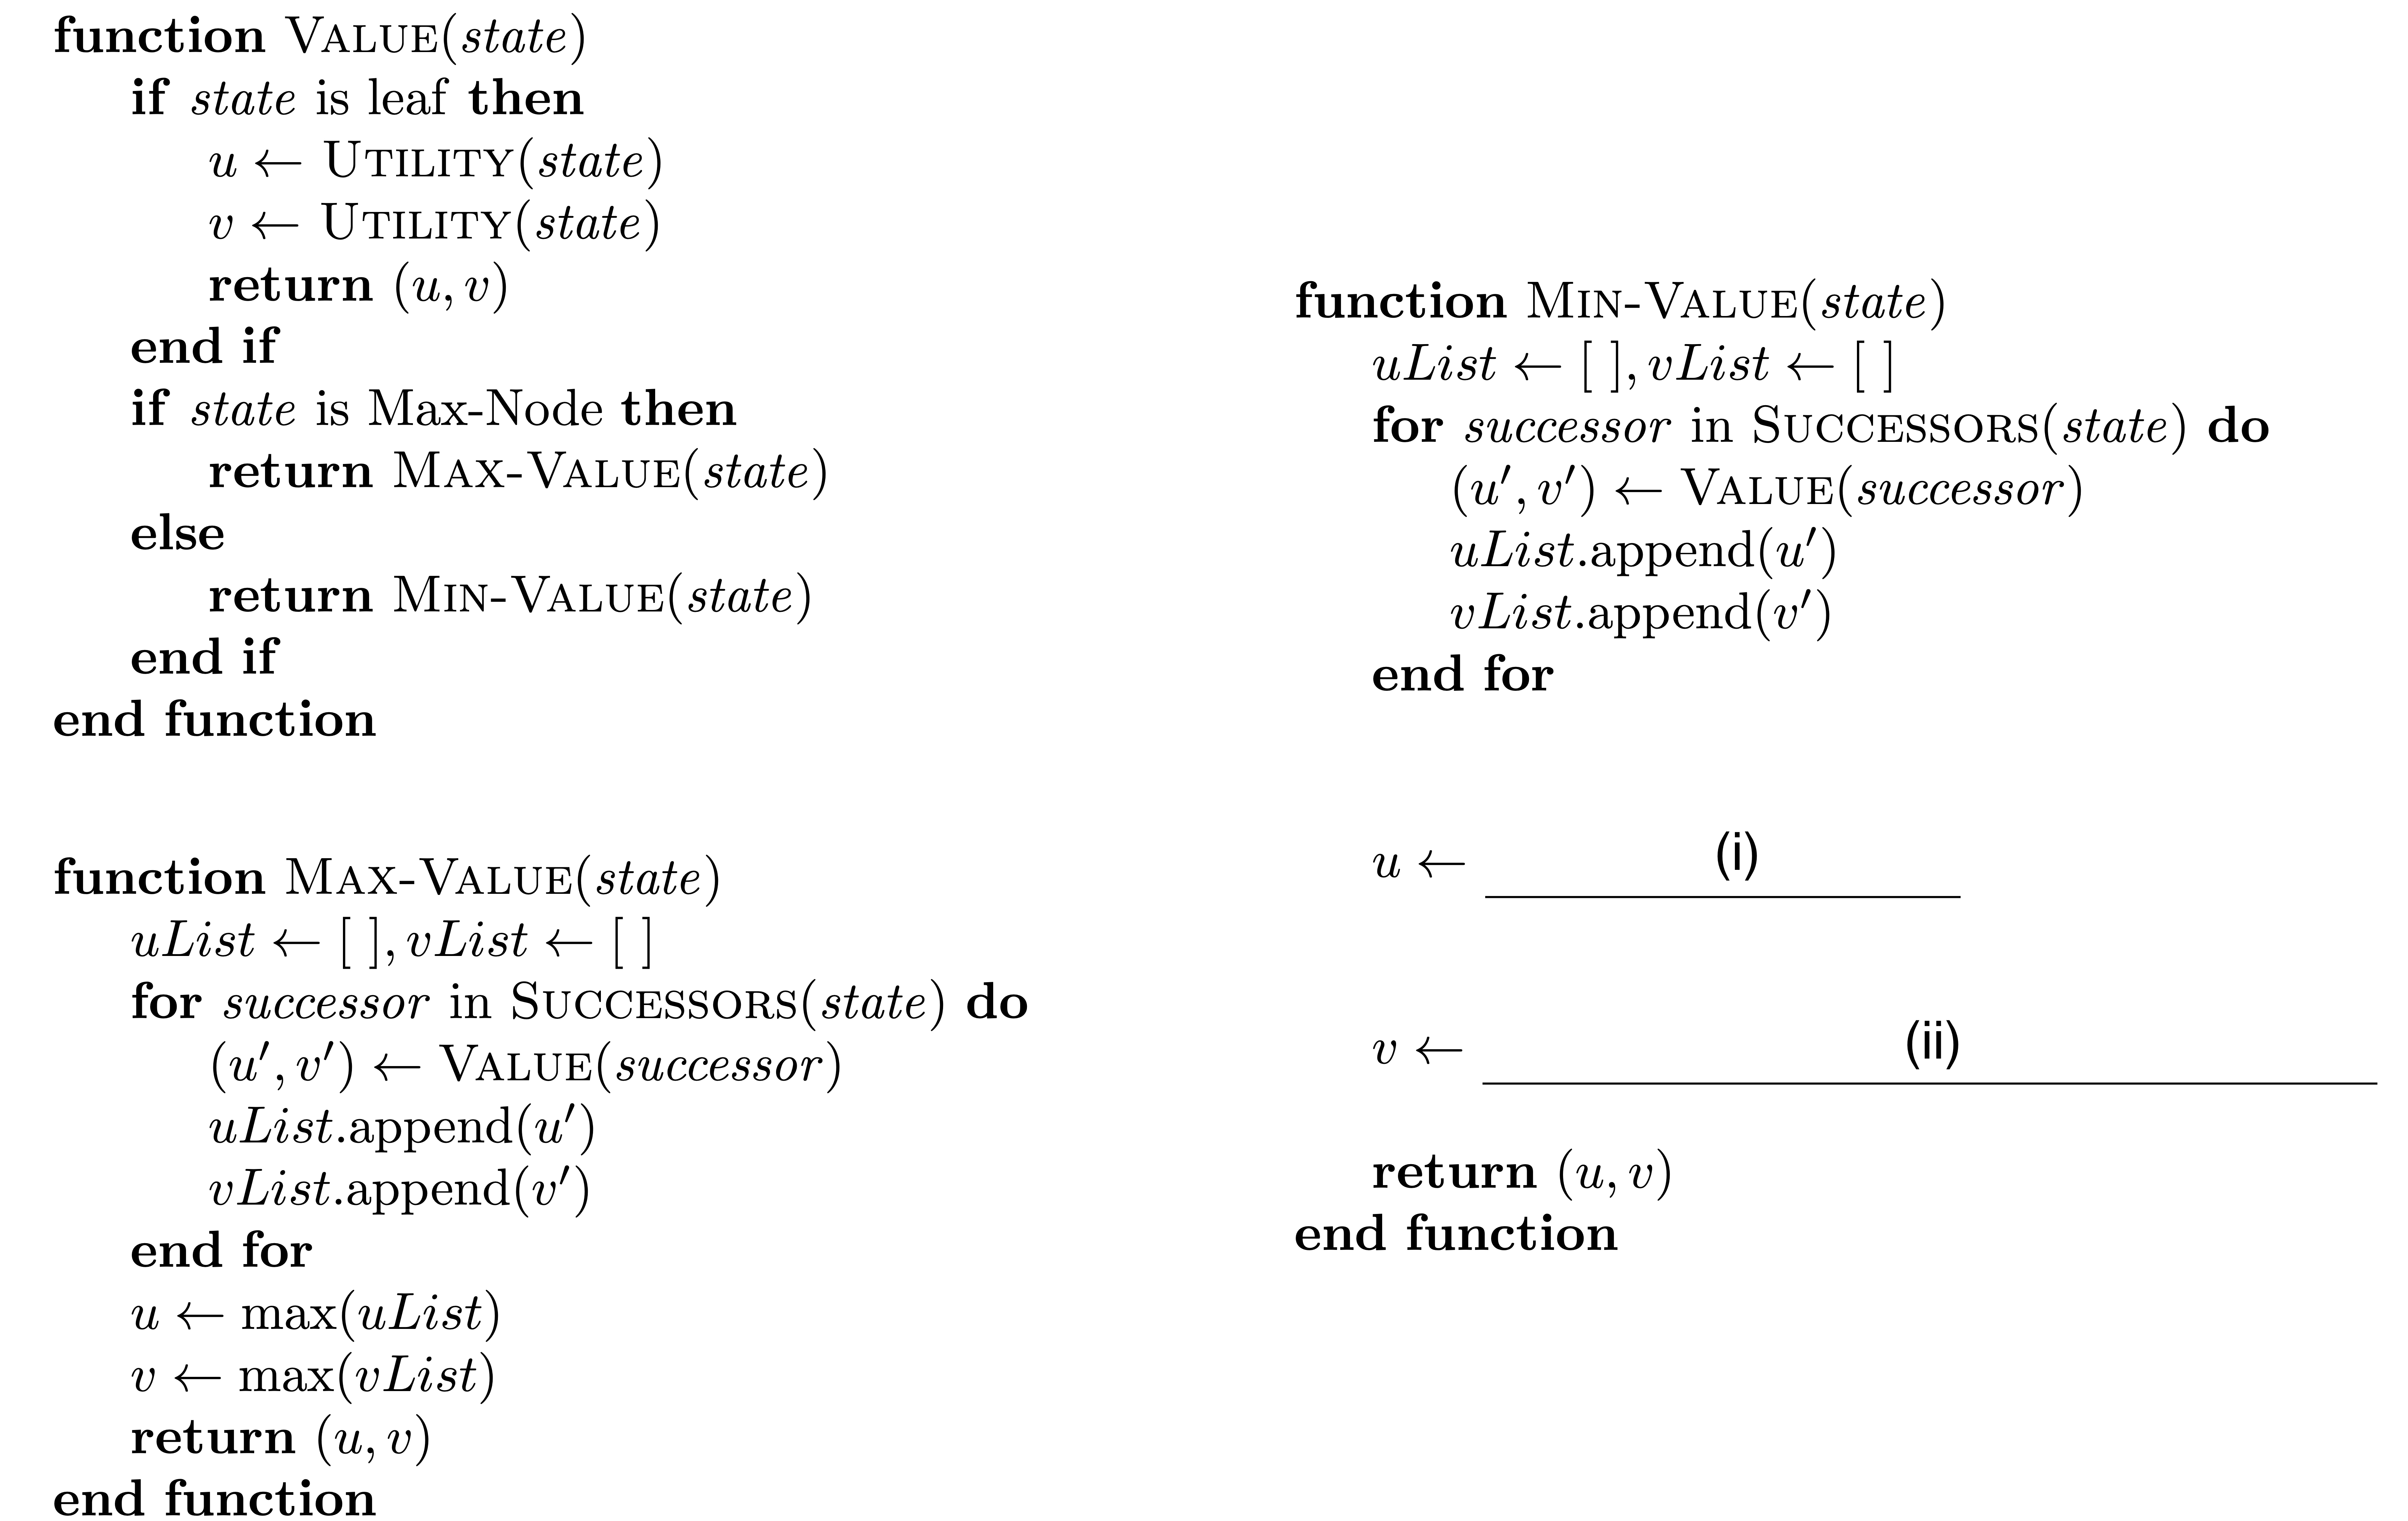
\includegraphics[width=1.\textwidth]{assignment3_3.jpg}
    \centering
    \end{figure}


u ---- min(uList)
 
v ---- max(max(uList), min(vList))

The u value is if Pacman does not use his power in the game subtree hanging from the current min-node. The u value is equal to the minimum of the u values of the children of the node.

The v value is when pacman uses his power once in the subtree. Pacman only has two options to use the power on the current node or to use the power further
down in the subtree.
  
\end{enumerate}


\newpage
\section*{Problem 3 [70 pt]: Multi-agent Pacman}
This is a programming problem adapted from CSCE 580 in Spring 2019.
Please use the following link for the problem specification:
\url{https://pooyanjamshidi.github.io/csce580/project2/}.

You need to submit 1) a .zip file containing the multiAgents.py file you edited, and 2) a .html file generated by the following command:
\texttt{python autograder.py --edx-output}

The .html file contains the autograder's results. 

\end{document}